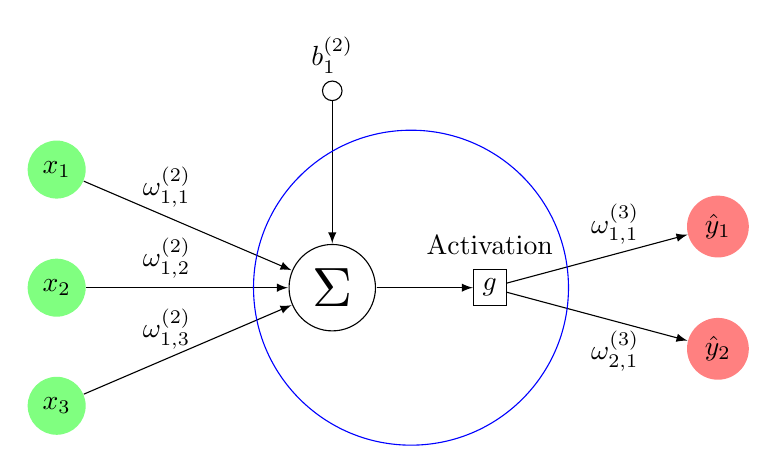
\begin{tikzpicture}[>=latex]
    \path
    % Summation
    (0,0)     node[circle,draw,scale=2,inner sep=2pt] (summation) {$\Sigma$}

    % Bias node
    +(90:2.5) node[circle,draw,inner sep=2.5pt] (bias) {}
              node[above=1mm] {$b_1^{(2)}$}
    % Input nodes
    +(-3.5,1.5)  node[circle,fill=green!50]  (input1) {$x_1$}
    +(-3.5,0)    node[circle,fill=green!50]  (input2) {$x_2$}
    +(-3.5,-1.5) node[circle,fill=green!50]  (input3) {$x_3$}

    % Activation function
    (2,0)    node[draw] (activation) {$g$} node[above=3mm]{Activation}

    % Output nodes
    +(15:3)  node[circle,fill=red!50]  (output1) {$\hat{y}_1$}
    +(-15:3) node[circle,fill=red!50]  (output2) {$\hat{y}_2$};

    % Link the different parts of the graph
    \draw[->] (summation)--(activation);
    \draw[->] (bias)--(summation);
    \draw[->] (activation)--(output1) node[pos=.6,above]{$\omega_{1,1}^{(3)}$};
    \draw[->] (activation)--(output2) node[pos=.6,below]{$\omega_{2,1}^{(3)}$};
    \draw[->] (input1)--(summation) node[pos=.4,above]{$\omega_{1,1}^{(2)}$};
    \draw[->] (input2)--(summation) node[pos=.4,above]{$\omega_{1,2}^{(2)}$};
    \draw[->] (input3)--(summation) node[pos=.4,above]{$\omega_{1,3}^{(2)}$};
    \draw[blue] (1,0) circle(2);
\end{tikzpicture}